\documentclass[12pt]{article}

%%%%%%%%%%%%%%%%%%%%%%%%%%%%
%%%%%%%%%%%%%%%%%%%%%%%%%%%%
% Load in packages
\usepackage{amsmath}
\usepackage{float}
\usepackage{amssymb}
\usepackage{hyperref}
\usepackage{graphicx}
\usepackage{enumitem}
\usepackage[top=1in, bottom=1in, left=1in, right=1in]{geometry}

% Graphs
\usepackage{pgfplots}
\pgfplotsset{compat=1.18}

% Toggleable solutions environment
\usepackage{comment}
\newif\ifsolutions
\solutionstrue     % change to \solutionsfalse to hide solutions

\ifsolutions
  \newenvironment{solution}{\par\noindent\textbf{Solution.}\par}{\vspace{1em}}
\else
  \excludecomment{solution}
\fi

%%%%%%%%%%%%%%%%%%%%%%%%%%%%
%%%%%%%%%%%%%%%%%%%%%%%%%%%%

\begin{document}

\begin{center}
\Large Import Tariffs and Export Duties

\medskip

\normalsize Elements of Microeconomics (discussion section 1)

\medskip

\small Rudy Kretschmar
\end{center}

\section*{Question 1}
Narnia is a large land that is far, far away. During the reign of the White Witch, 
the land produces and consumes Turkish Delight. The world price of Turkish Delight 
is \$2 per bag.

Narnia's demand and supply for Turkish Delight are governed by the following equations:
\begin{align*}
    Q_D &= 8 - P \\
    Q_S &= P
\end{align*}
where $P$ is measured in dollars per bag and $Q$ is measured in bags.

\begin{enumerate}[label=(\alph*)]
\item Draw a well-labeled graph of this market if Narnia does not allow trade. 
Calculate the equilibrium price and quantity, consumer surplus, producer surplus, 
and total surplus.
\begin{solution}

\begin{center}
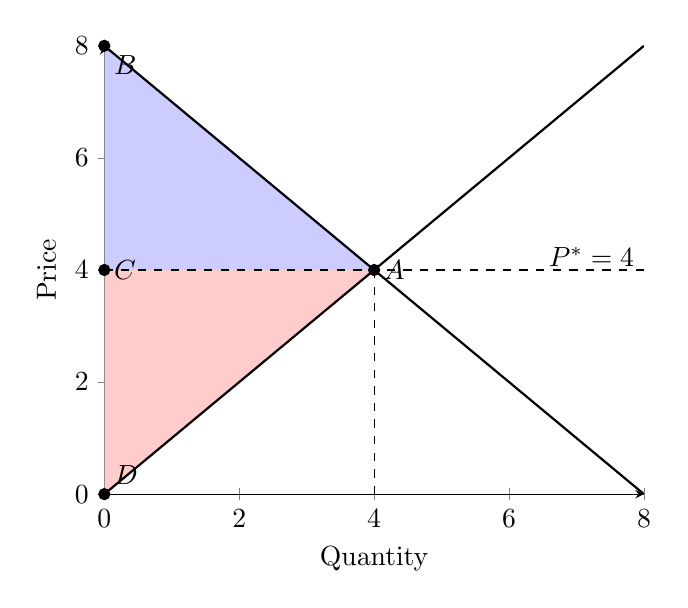
\begin{tikzpicture}
\begin{axis}[
axis lines=left,
xlabel={Quantity},
ylabel={Price},
xmin=0,xmax=8,
ymin=0,ymax=8,
samples=100
]

% Consumer surplus shading
\addplot[
fill=blue!20,
draw=none
] coordinates {(0,8) (0,4) (4,4) (0,8)};

% Producer surplus shading
\addplot[
fill=red!20,
draw=none
] coordinates {(0,0) (0,4) (4,4) (0,0)};

% Demand and Supply
\addplot[thick, domain=0:8] {8-x};
\addplot[thick, domain=0:8] {x};

% Equilibrium guides
\addplot[dashed] coordinates {(4,0) (4,4)};
\addplot[dashed] coordinates {(0,4) (8,4)};
\node[anchor=south east, fill=white, inner sep=1pt] at (axis cs:7.9,4) {$P^*=4$};

% Points
\addplot[mark=*] coordinates {(4,4)} node[right] {$A$};
\addplot[mark=*] coordinates {(0,8)} node[below right] {$B$};
\addplot[mark=*] coordinates {(0,4)} node[right] {$C$};
\addplot[mark=*] coordinates {(0,0)} node[above right] {$D$};


\end{axis}
\end{tikzpicture}
\end{center}

In autarky, equilibrium occurs where demand equals supply: 

$$8 - P = P \rightarrow P^* = 4, \quad Q^* = 4$$, 

where $Q^*$ is most easily solved in the supply equation. Point $A=(4,4)$ represents the market equilibrium.

\medskip

Consumer surplus corresponds to triangle $BCA$. Note that $CA$ is the equilibrium quantity and $BC$ is solved by differencing the y-intercept of the demand equation with the equilibrium price.

$$
CS = \frac{1}{2}\times BC \times CA = \frac 1 2 \times (8-4) \times 4 = 8
$$


\medskip

Producer surplus corresponds to triangle $DCA$. Note that $CA$ is the equilibrium quantity and $DC$ is solved by differencing the y-intercept of the supply equation with the equilibrium price.

$$
PS = \frac{1}{2}\times DC \times CA = \frac 1 2 \times (4-0) \times 4 = 8
$$


\medskip

Total surplus is

$$
TS = CS + PS = 8 + 8 = 16.
$$

\end{solution}

\item Narnia then opens the market to trade at the world price. Draw another graph 
to describe the new situation in the Turkish Delight market. Calculate the domestic 
price, quantities of consumption and production, imports, consumer surplus, 
producer surplus, total surplus, and the gains from trade.

\begin{solution}

\begin{center}
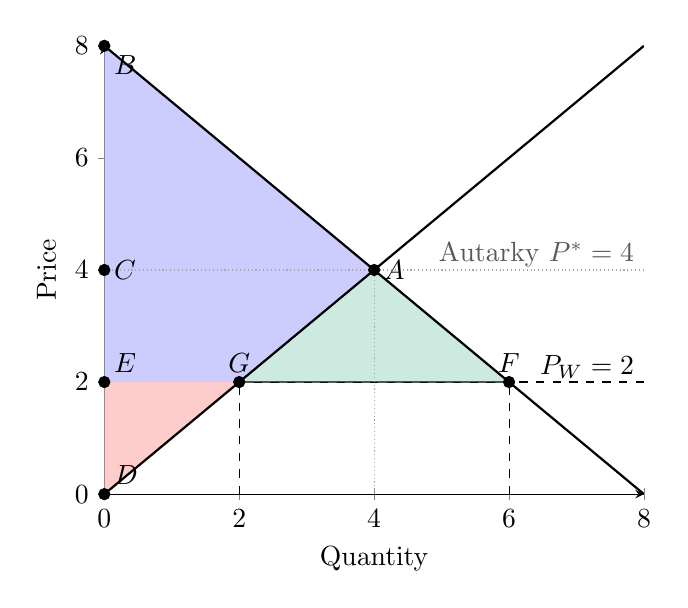
\begin{tikzpicture}
\begin{axis}[
axis lines=left,
xlabel={Quantity},
ylabel={Price},
xmin=0,xmax=8,
ymin=0,ymax=8,
samples=100
]

% World price line
\addplot[dashed] coordinates {(0,2) (8,2)};
\node[anchor=south east, fill=white, inner sep=1pt] at (axis cs:7.9,2) {$P_W=2$};

% Consumer surplus shading (triangle between demand and Pw from Q=0 to Q=6)
\addplot[
fill=blue!20,
draw=none
] coordinates {(0,8) (0,2) (6,2) (0,8)};

% Producer surplus shading (triangle under Pw above supply from Q=0 to Q=2)
\addplot[
fill=red!20,
draw=none
] coordinates {(0,0) (2,2) (0,2) (0,0)};

% Gains from trade triangle (AGF)
\addplot[
  fill=green!20,
  fill opacity=0.6,
  draw=black
] coordinates {(2,2) (4,4) (6,2) (2,2)};

% Demand and Supply
\addplot[thick, domain=0:8] {8-x};
\addplot[thick, domain=0:8] {x};

% Quantity guides at world price
\addplot[dashed] coordinates {(2,0) (2,2)};
\addplot[dashed] coordinates {(6,0) (6,2)};

% Autarky equilibrium guides (reference)
\addplot[densely dotted, gray!70] coordinates {(4,0) (4,4)};
\addplot[densely dotted, gray!70] coordinates {(0,4) (8,4)};
\node[anchor=south east, fill=white, inner sep=1pt, text=gray!70!black] at (axis cs:7.9,4) {Autarky $P^*=4$};

% Key points
\addplot[mark=*] coordinates {(4,4)} node[right] {$A$};
\addplot[mark=*] coordinates {(0,8)} node[below right] {$B$};
\addplot[mark=*] coordinates {(0,4)} node[right] {$C$};
\addplot[mark=*] coordinates {(0,0)} node[above right] {$D$};
\addplot[mark=*] coordinates {(0,2)} node[above right] {$E$};   % world price on y-axis
\addplot[mark=*] coordinates {(6,2)} node[above] {$F$};         % consumption at Pw
\addplot[mark=*] coordinates {(2,2)} node[above] {$G$};         % production at Pw


\end{axis}
\end{tikzpicture}
\end{center}

\newpage
Under free trade, the domestic price equals the world price:
$$
P_W = 2.
$$

Domestic consumption is determined by demand at $P_W$:
$$
Q_D(P_W) = 8 - 2 = 6,
$$
so point $F=(6,2)$ is consumption at the world price.

Domestic production is determined by supply at $P_W$:
$$
Q_S(P_W) = 2,
$$
so point $G=(2,2)$ is production at the world price.

Imports equal the horizontal gap between consumption and production at $P_W$:
$$
M = Q_D - Q_S = 6 - 2 = 4.
$$

\medskip

Consumer surplus corresponds to triangle $BEF$, where $EF$ is the quantity consumed at the world price and $BE$ is the vertical distance between points $B=(0,8)$ and $E=(0,2)$:
$$
CS = \frac{1}{2}\times BE \times EF.
$$
$$
BE = 8-2 = 6,\qquad EF = 6.
$$
$$
CS = \tfrac12 (6)(6) = 18.
$$

\medskip

Producer surplus corresponds to triangle $OEG$, where $O=(0,0)$, $EG$ is the quantity produced at the world price, and $OE$ is the world price:
$$
PS = \frac{1}{2}\times OE \times EG.
$$
$$
OE = 2,\qquad EG = 2.
$$
$$
PS = \tfrac12 (2)(2) = 2.
$$

\medskip

Total surplus under free trade is
$$
TS = CS + PS = 18 + 2 = 20.
$$

Gains from trade are the increase in total surplus relative to autarky. Alternatively, one can find the area taken in the green triangle $AGE$: 
$$
GFT = 20 - 16 = 4.
$$



\end{solution}

\item After a while, the White Witch imposes a \$1 per bag tariff on imported 
Turkish Delight in response to the pleas of Narnian sweet-makers. On a graph, 
show the effects of this tariff. Calculate the domestic price, quantities of 
consumption and production, imports, consumer surplus, producer surplus, 
government revenue, total surplus, and the resulting deadweight loss.

\begin{solution}

\begin{center}
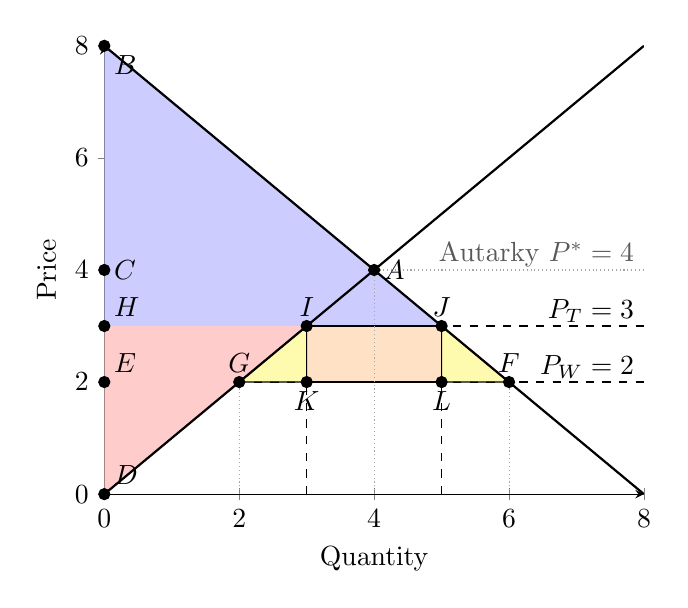
\begin{tikzpicture}
\begin{axis}[
axis lines=left,
xlabel={Quantity},
ylabel={Price},
xmin=0,xmax=8,
ymin=0,ymax=8,
samples=100
]

% World price and tariff-inclusive domestic price
\addplot[dashed] coordinates {(0,2) (8,2)};
\node[anchor=south east, fill=white, inner sep=1pt] at (axis cs:7.9,2) {$P_W=2$};

\addplot[dashed] coordinates {(0,3) (8,3)};
\node[anchor=south east, fill=white, inner sep=1pt] at (axis cs:7.9,3) {$P_T=3$};

% Autarky equilibrium price (reference)
\addplot[densely dotted, gray!70] coordinates {(0,4) (8,4)};
\node[anchor=south east, fill=white, inner sep=1pt, text=gray!70!black] at (axis cs:7.9,4) {Autarky $P^*=4$};

% Consumer surplus under tariff
\addplot[
fill=blue!20,
draw=none
] coordinates {(0,8) (0,3) (5,3) (0,8)};

% Producer surplus under tariff
\addplot[
fill=red!20,
draw=none
] coordinates {(0,0) (0,3) (3,3) (0,0)};

% Tariff revenue rectangle
\addplot[
fill=orange!35,
draw=black,
fill opacity=0.65
] coordinates {(3,2) (3,3) (5,3) (5,2) (3,2)};

% Deadweight loss triangles
\addplot[
fill=yellow!45,
draw=black,
fill opacity=0.7
] coordinates {(2,2) (3,2) (3,3) (2,2)};
\addplot[
fill=yellow!45,
draw=black,
fill opacity=0.7
] coordinates {(5,3) (5,2) (6,2) (5,3)};

% Demand and Supply
\addplot[thick, domain=0:8] {8-x};
\addplot[thick, domain=0:8] {x};

% Quantity guides under tariff
\addplot[dashed] coordinates {(3,0) (3,3)};
\addplot[dashed] coordinates {(5,0) (5,3)};

% Free-trade quantities (reference)
\addplot[densely dotted, gray!70] coordinates {(2,0) (2,2)};
\addplot[densely dotted, gray!70] coordinates {(6,0) (6,2)};
\addplot[densely dotted, gray!70] coordinates {(4,0) (4,4)};

% Key points
\addplot[mark=*] coordinates {(4,4)} node[right] {$A$};
\addplot[mark=*] coordinates {(0,8)} node[below right] {$B$};
\addplot[mark=*] coordinates {(0,4)} node[right] {$C$};
\addplot[mark=*] coordinates {(0,0)} node[above right] {$D$};
\addplot[mark=*] coordinates {(0,2)} node[above right] {$E$};
\addplot[mark=*] coordinates {(0,3)} node[above right] {$H$};
\addplot[mark=*] coordinates {(2,2)} node[above] {$G$};
\addplot[mark=*] coordinates {(6,2)} node[above] {$F$};
\addplot[mark=*] coordinates {(3,3)} node[above] {$I$};
\addplot[mark=*] coordinates {(5,3)} node[above] {$J$};
\addplot[mark=*] coordinates {(3,2)} node[below] {$K$};
\addplot[mark=*] coordinates {(5,2)} node[below] {$L$};



\end{axis}
\end{tikzpicture}
\end{center}

With a specific tariff $t=1$, the domestic price rises above the world price by the tariff amount:
$$
P_T = P_W + t = 2 + 1 = 3.
$$

At $P_T=3$:
$$
Q_D(P_T)=8-3=5,\qquad Q_S(P_T)=3.
$$
So $I=(3,3)$ and $J=(5,3)$. Their intersections with the world-price line $P_W=2$ are $K=(3,2)$ and $L=(5,2)$.

Imports fall to
$$
M_T = Q_D - Q_S = 5-3=2.
$$

\medskip

Consumers pay the price with the tariff, hence why the demand is calculated with that price. Consumer surplus is triangle $BHJ$, with vertices $B=(0,8)$, $H=(0,3)$, and $J=(5,3)$:
$$
CS_T=\tfrac12(8-3)(5)=\tfrac12(5)(5)=12.5.
$$

Producer surplus is triangle $DHI$, with vertices $D=(0,0)$, $H=(0,3)$, and $I=(3,3)$:
$$
PS_T=\tfrac12(3-0)(3)=\tfrac12(3)(3)=4.5.
$$

Government tariff revenue is rectangle $IKLJ$, with vertices $I=(3,3)$, $K=(3,2)$, $L=(5,2)$, and $J=(5,3)$:
$$
GR=t\cdot M_T = 1\cdot 2 = 2.
$$

Total surplus with the tariff is
$$
TS_T=CS_T+PS_T+GR=12.5+4.5+2=19.
$$

Deadweight loss is the reduction in total surplus relative to free trade ($TS_{FT}=20$):
$$
DWL=TS_{FT}-TS_T=20-19=1.
$$
Equivalently, DWL is the sum of triangles $GKI$ and $LJF$, with vertices
$G=(2,2),K=(3,2),I=(3,3)$ and $L=(5,2),J=(5,3),F=(6,2)$.
Each has area $\tfrac12(1)(1)=0.5$, totaling $1$.

\end{solution}

\item What are the gains from opening up trade? What are the deadweight losses 
from restricting trade with the tariff? Who benefits under each policy? Who incurs a loss? 
Give both graphical and numerical answers.
\begin{solution}
From autarky to free trade (part b), total surplus rises from $16$ to $20$, so the
gains from trade are
$$
GFT = 20-16=4.
$$
Graphically, this is triangle $AGE$ in part (b).

\medskip

Distribution of gains/losses from opening to trade:
$$
\Delta CS = 18-8 = +10,\qquad
\Delta PS = 2-8 = -6.
$$
So consumers gain, producers lose, and the nation gains $+4$ overall.

\medskip

From free trade to tariff (part c), total surplus falls from $20$ to $19$, so deadweight loss is
$$
DWL = 20-19=1.
$$
Graphically, this is the sum of the two small yellow triangles in part (c).

\medskip

Distribution of gains/losses from imposing the tariff (relative to free trade):
$$
\Delta CS = 12.5-18 = -5.5,\qquad
\Delta PS = 4.5-2 = +2.5,\qquad
\Delta GR = 2-0 = +2.
$$
Consumers lose, domestic producers gain, and the government gains tariff revenue.
The net national effect is $-1$, which is exactly the deadweight loss.
\end{solution}
\end{enumerate}

\clearpage
\section*{Question 2}

Parma is another land that is far, far away. Parma is ruled by King Giovanni, and the land both produces and consumes jawns. Parma's demand and supply of jawns are given by the following equations:
\begin{align*}
    Q_D &= 10 - \frac 1 2 P \\
    Q_S &= 2P
\end{align*}

where $P$ is measured in dollars per bag and $Q$ is measured in flat units.

\begin{enumerate}[label=(\alph*)]

\item Draw a well-labeled graph of this market if Parma does not allow trade. 
Calculate the equilibrium price and quantity, consumer surplus, producer surplus, 
and total surplus.
\begin{solution}

\begin{center}
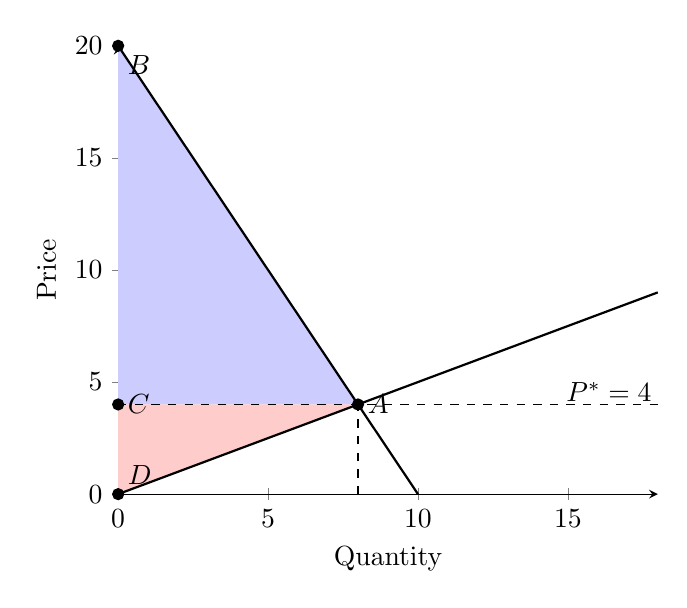
\begin{tikzpicture}
\begin{axis}[
axis lines=left,
xlabel={Quantity},
ylabel={Price},
xmin=0,xmax=18,
ymin=0,ymax=20,
samples=100
]

% Consumer surplus shading
\addplot[
fill=blue!20,
draw=none
] coordinates {(0,20) (0,4) (8,4) (0,20)};

% Producer surplus shading
\addplot[
fill=red!20,
draw=none
] coordinates {(0,0) (0,4) (8,4) (0,0)};

% Demand and Supply
\addplot[thick, domain=0:10] {20-2*x};
\addplot[thick, domain=0:18] {0.5*x};

% Equilibrium guides
\addplot[dashed] coordinates {(8,0) (8,4)};
\addplot[dashed] coordinates {(0,4) (18,4)};
\node[anchor=south east, fill=white, inner sep=1pt] at (axis cs:17.9,4) {$P^*=4$};

% Points
\addplot[mark=*] coordinates {(8,4)} node[right] {$A$};
\addplot[mark=*] coordinates {(0,20)} node[below right] {$B$};
\addplot[mark=*] coordinates {(0,4)} node[right] {$C$};
\addplot[mark=*] coordinates {(0,0)} node[above right] {$D$};


\end{axis}
\end{tikzpicture}
\end{center}

In autarky, equilibrium occurs where demand equals supply:

$$
10-\frac{1}{2}P = 2P \rightarrow 10=\frac{5}{2}P \rightarrow P^*=4,\quad Q^*=8,
$$
where $Q^*$ is most easily solved in the supply equation. Point $A=(8,4)$ represents the market equilibrium.

\medskip

Consumer surplus corresponds to triangle $BCA$. Note that $CA$ is the equilibrium quantity and $BC$ is solved by differencing the y-intercept of the demand equation with the equilibrium price.
$$
CS = \frac{1}{2}\times BC \times CA = \frac{1}{2}\times(20-4)\times 8 = 64.
$$

\medskip

Producer surplus corresponds to triangle $DCA$. Note that $CA$ is the equilibrium quantity and $DC$ is solved by differencing the y-intercept of the supply equation with the equilibrium price.
$$
PS = \frac{1}{2}\times DC \times CA = \frac{1}{2}\times(4-0)\times 8 = 16.
$$

\medskip

Total surplus is
$$
TS = CS + PS = 64 + 16 = 80.
$$

\end{solution}

\item Parma then opens the market to international trade. The world price of jawns 
is $P_W = 8$. Draw another graph to describe the new situation in the Parmese 
jawn market. Calculate the domestic price, quantities of consumption and 
production, exports, consumer surplus, producer surplus, total surplus, 
and the gains from trade.
\begin{solution}

\begin{center}
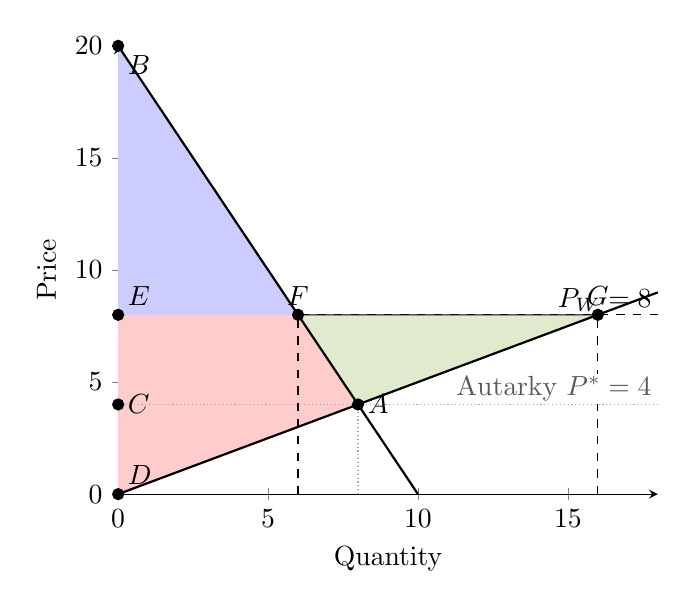
\begin{tikzpicture}
\begin{axis}[
axis lines=left,
xlabel={Quantity},
ylabel={Price},
xmin=0,xmax=18,
ymin=0,ymax=20,
samples=100
]

% World price line
\addplot[dashed] coordinates {(0,8) (18,8)};
\node[anchor=south east, fill=white, inner sep=1pt] at (axis cs:17.9,8) {$P_W=8$};

% Consumer surplus shading
\addplot[
fill=blue!20,
draw=none
] coordinates {(0,20) (0,8) (6,8) (0,20)};

% Producer surplus shading
\addplot[
fill=red!20,
draw=none
] coordinates {(0,0) (16,8) (0,8) (0,0)};

% Gains from trade triangle (AFG)
\addplot[
fill=green!20,
fill opacity=0.6,
draw=black
] coordinates {(6,8) (8,4) (16,8) (6,8)};

% Demand and Supply
\addplot[thick, domain=0:10] {20-2*x};
\addplot[thick, domain=0:18] {0.5*x};

% Quantity guides at world price
\addplot[dashed] coordinates {(6,0) (6,8)};
\addplot[dashed] coordinates {(16,0) (16,8)};

% Autarky equilibrium guides (reference)
\addplot[densely dotted, gray!70] coordinates {(8,0) (8,4)};
\addplot[densely dotted, gray!70] coordinates {(0,4) (18,4)};
\node[anchor=south east, fill=white, inner sep=1pt, text=gray!70!black] at (axis cs:17.9,4) {Autarky $P^*=4$};

% Key points
\addplot[mark=*] coordinates {(8,4)} node[right] {$A$};
\addplot[mark=*] coordinates {(0,20)} node[below right] {$B$};
\addplot[mark=*] coordinates {(0,4)} node[right] {$C$};
\addplot[mark=*] coordinates {(0,0)} node[above right] {$D$};
\addplot[mark=*] coordinates {(0,8)} node[above right] {$E$};
\addplot[mark=*] coordinates {(6,8)} node[above] {$F$};
\addplot[mark=*] coordinates {(16,8)} node[above] {$G$};


\end{axis}
\end{tikzpicture}
\end{center}

Under free trade, the domestic price equals the world price:
$$
P_W = 8.
$$

Domestic consumption is determined by demand at $P_W$:
$$
Q_D(P_W)=10-\frac{1}{2}(8)=6,
$$
so point $F=(6,8)$ is consumption at the world price.

Domestic production is determined by supply at $P_W$:
$$
Q_S(P_W)=2(8)=16,
$$
so point $G=(16,8)$ is production at the world price.

Exports equal the horizontal gap between production and consumption at $P_W$:
$$
X = Q_S - Q_D = 16-6=10.
$$

\medskip

Consumer surplus corresponds to triangle $BEF$, where $EF$ is the quantity consumed at the world price and $BE$ is the vertical distance between points $B=(0,20)$ and $E=(0,8)$:
$$
CS = \frac{1}{2}\times BE \times EF.
$$
$$
BE = 20-8=12,\qquad EF = 6.
$$
$$
CS = \tfrac12 (12)(6) = 36.
$$

\medskip

Producer surplus corresponds to triangle $OEG$, where $O=(0,0)$, $EG$ is the quantity produced at the world price, and $OE$ is the world price:
$$
PS = \frac{1}{2}\times OE \times EG.
$$
$$
OE = 8,\qquad EG = 16.
$$
$$
PS = \tfrac12 (8)(16) = 64.
$$

\medskip

Total surplus under free trade is
$$
TS = CS + PS = 36 + 64 = 100.
$$

Gains from trade are the increase in total surplus relative to autarky. Alternatively, one can find the area taken in the green triangle $AFG$:
$$
GFT = 100 - 80 = 20.
$$

\end{solution}

\item After hearing complaints from his dear friend Yianni about the dearth of jawns,
King Giovanni imposes a \$2 per unit \textbf{export duty} on jawns leaving Parma. 
On a graph, show the effects of this export duty. Calculate the domestic price, 
quantities of consumption and production, exports, consumer surplus, 
producer surplus, government revenue, and total surplus.
\begin{solution}

\begin{center}
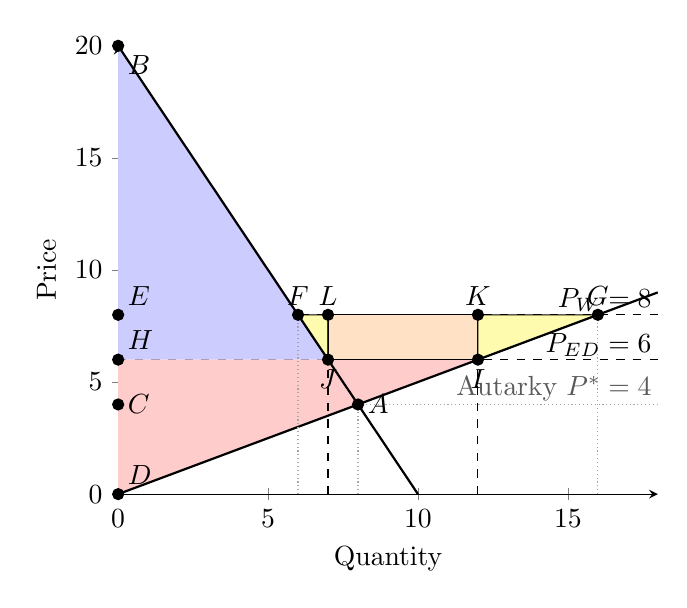
\begin{tikzpicture}
\begin{axis}[
axis lines=left,
xlabel={Quantity},
ylabel={Price},
xmin=0,xmax=18,
ymin=0,ymax=20,
samples=100
]

% World price and export-duty domestic price
\addplot[dashed] coordinates {(0,8) (18,8)};
\node[anchor=south east, fill=white, inner sep=1pt] at (axis cs:17.9,8) {$P_W=8$};

\addplot[dashed] coordinates {(0,6) (18,6)};
\node[anchor=south east, fill=white, inner sep=1pt] at (axis cs:17.9,6) {$P_{ED}=6$};

% Autarky equilibrium price (reference)
\addplot[densely dotted, gray!70] coordinates {(0,4) (18,4)};
\node[anchor=south east, fill=white, inner sep=1pt, text=gray!70!black] at (axis cs:17.9,4) {Autarky $P^*=4$};

% Consumer surplus under export duty
\addplot[
fill=blue!20,
draw=none
] coordinates {(0,20) (0,6) (7,6) (0,20)};

% Producer surplus under export duty
\addplot[
fill=red!20,
draw=none
] coordinates {(0,0) (0,6) (12,6) (0,0)};

% Export-duty revenue rectangle
\addplot[
fill=orange!35,
draw=black,
fill opacity=0.65
] coordinates {(7,6) (7,8) (12,8) (12,6) (7,6)};

% Deadweight loss triangles
\addplot[
fill=yellow!45,
draw=black,
fill opacity=0.7
] coordinates {(6,8) (7,8) (7,6) (6,8)};
\addplot[
fill=yellow!45,
draw=black,
fill opacity=0.7
] coordinates {(12,6) (12,8) (16,8) (12,6)};

% Demand and Supply
\addplot[thick, domain=0:10] {20-2*x};
\addplot[thick, domain=0:18] {0.5*x};

% Quantity guides under export duty
\addplot[dashed] coordinates {(7,0) (7,6)};
\addplot[dashed] coordinates {(12,0) (12,6)};

% Free-trade quantities (reference)
\addplot[densely dotted, gray!70] coordinates {(6,0) (6,8)};
\addplot[densely dotted, gray!70] coordinates {(16,0) (16,8)};
\addplot[densely dotted, gray!70] coordinates {(8,0) (8,4)};

% Key points
\addplot[mark=*] coordinates {(8,4)} node[right] {$A$};
\addplot[mark=*] coordinates {(0,20)} node[below right] {$B$};
\addplot[mark=*] coordinates {(0,4)} node[right] {$C$};
\addplot[mark=*] coordinates {(0,0)} node[above right] {$D$};
\addplot[mark=*] coordinates {(0,8)} node[above right] {$E$};
\addplot[mark=*] coordinates {(0,6)} node[above right] {$H$};
\addplot[mark=*] coordinates {(6,8)} node[above] {$F$};
\addplot[mark=*] coordinates {(16,8)} node[above] {$G$};
\addplot[mark=*] coordinates {(12,6)} node[below] {$I$};
\addplot[mark=*] coordinates {(7,6)} node[below] {$J$};
\addplot[mark=*] coordinates {(12,8)} node[above] {$K$};
\addplot[mark=*] coordinates {(7,8)} node[above] {$L$};


\end{axis}
\end{tikzpicture}
\end{center}

With a specific export duty $t=2$, the domestic price in Parma falls below the world price by the duty amount:
$$
P_{ED} = P_W - t = 8 - 2 = 6.
$$

At $P_{ED}=6$:
$$
Q_D(P_{ED})=10-\frac{1}{2}(6)=7,\qquad Q_S(P_{ED})=2(6)=12.
$$
So $J=(7,6)$ and $I=(12,6)$. Their intersections with the world-price line $P_W=8$ are $L=(7,8)$ and $K=(12,8)$.

Exports fall to
$$
X_{ED} = Q_S - Q_D = 12-7=5.
$$

\medskip

Consumer surplus is triangle $BHJ$, with vertices $B=(0,20)$, $H=(0,6)$, and $J=(7,6)$:
$$
CS_{ED}=\tfrac12(20-6)(7)=\tfrac12(14)(7)=49.
$$

Producer surplus is triangle $DHI$, with vertices $D=(0,0)$, $H=(0,6)$, and $I=(12,6)$:
$$
PS_{ED}=\tfrac12(6-0)(12)=\tfrac12(6)(12)=36.
$$

Government revenue is rectangle $JLKI$, with vertices $J=(7,6)$, $L=(7,8)$, $K=(12,8)$, and $I=(12,6)$:
$$
GR=t\cdot X_{ED} = 2\cdot 5 = 10.
$$

Total surplus with the export duty is
$$
TS_{ED}=CS_{ED}+PS_{ED}+GR=49+36+10=95.
$$

\end{solution}

\item What are the gains from opening up trade? What are the deadweight losses 
from restricting trade with the export duty? Who benefits under each policy? 
Who incurs a loss? Give both graphical and numerical answers.
\begin{solution}
From autarky to free trade (part b), total surplus rises from $80$ to $100$, so the
gains from trade are
$$
GFT = 100-80=20.
$$
Graphically, this is triangle $AFG$ in part (b).

\medskip

Distribution of gains/losses from opening to trade:
$$
\Delta CS = 36-64 = -28,\qquad
\Delta PS = 64-16 = +48.
$$
So consumers lose, producers gain, and the nation gains $+20$ overall.

\medskip

From free trade to export duty (part c), total surplus falls from $100$ to $95$, so deadweight loss is
$$
DWL = 100-95=5.
$$
Graphically, this is the sum of the two small yellow triangles in part (c).

\medskip

Distribution of gains/losses from imposing the export duty (relative to free trade):
$$
\Delta CS = 49-36 = +13,\qquad
\Delta PS = 36-64 = -28,\qquad
\Delta GR = 10-0 = +10.
$$
Consumers gain from the lower domestic price, producers lose, and the government gains export-duty revenue.
The net national effect is $-5$, which is exactly the deadweight loss.
\end{solution}

\end{enumerate}


\end{document}
